
\section{Deep Learning}
The goal of this section/lecture is to introduce the multilayer perceptron (MLP) model and to explain the training algorithm for an MLP.\\
$ $\\
Until now our model has been define as 
\begin{align*} 
	\hat{y}\left(x\right) = w^{T}x
\end{align*}
In order to model data that weren't linearly 'correlated' we introduced feature expansion and kernel method (inherently) which map data to a different representation. The goal was to use a map $\phi\left(\cdot\right)$ in order to transform the input nonlinearly which gives more flexibility.\\
$ $\\
The issue with all of those were that all of those data processing strategies we have discussed so far were all manually designed (the transformation corresponding to a kernel is still defined manually). There is, however no guarantee that they are the best representations for the task at hand. Ideally, one would therefore like to learn the representation jointly with the classifier.

\begin{parag}{Motivating example: Curve fitting}
    In the 1D input and 1D output scenario, we would like to find a mapping from $x$ to $y$ that approximates the curve below.
	\begin{center}
	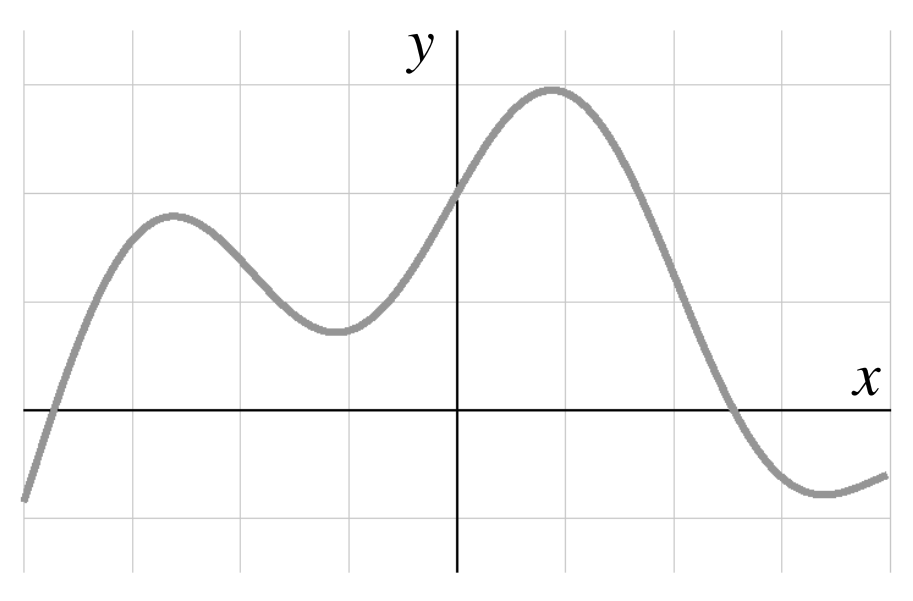
\includegraphics[scale=0.3]{screenshots/2026-04-21.png}
	\end{center}
	In previous lecture, we have attempted to do so by performing a polynomial feature expansion:
	\begin{align*} 
		x \to \begin{pmatrix} 1 \\ x \\ x^2 \\ \vdots \\ x^{M} \end{pmatrix} 
	\end{align*}
	We then applied a linear model to the expanded features. In this case, the feature expansion was manually defined, independently of the linear model training. Instead, we would like to learn the feature expansion and the linear model jointly.\\
	$ $\\
	To achieve this, we can define a parametric feature expansion strategy; as we like linear models, let's use one for this purpose. Naively, we could then write the mapping as:
	\begin{align*} 
		x \to W_{\left(1\right)}^{T}\begin{pmatrix} 1 \\ x \end{pmatrix} , \mathspace \text{with} W_{\left(1\right)} \in \mathbb{R}^{2 \times M}
	\end{align*}
	and then apply a linear model with parameters $W_{\left(2\right)} \in \mathbb{R}^{M \times 1}$ to the resulting representation to predict $y$.\\
	$ $\\
	However, as mentioned in a previous lecture, linear feature expansion is useless; you can achieve the same results with just one linear model. Therefore an interesting thing here would be to add \important{nonlineariry} in the process. To achieve this, we will use a nonlinear function $f: \mathbb{R} \to \mathbb{R}$. But before that we need to define on what this function will be applied.
	\begin{align*} 
		a_{\left(1\right)} =  W_{\left(1\right)}^{T} \begin{pmatrix} 1 \\ x \end{pmatrix}  = \begin{pmatrix} W_{\left(1\right)}^{\left(1, 0\right)} + W_{\left(1\right)}^{\left(1, 1\right)}x \\ W_{\left(1\right)}^{\left(2, 0\right)}  + W_{\left(1\right)}^{\left(2, 1\right)}x\\ \vdots \\ W_{\left(1\right)}^{\left(M, 0\right)} + W_{\left(1\right)}^{\left(M, 1\right)}x \end{pmatrix} = \begin{pmatrix} a_{\left(1\right)}^{\left(1\right)} \\ a_{\left(1\right)}^{\left(2\right)} \\ \vdots \\ a_{\left(1\right)}^{\left(M\right)} \end{pmatrix} 
	\end{align*}
	But first let us step back a bit and think on what we just did and \important{why} is it different (we will come back to this later).\\
	$ $\\
	Then, our parametric feature expansion process can be expressed as 
	\begin{align*} 
		x \to \begin{pmatrix} f\left(a_{\left(1\right)}^{\left(1\right)}\right) \\ f\left(a_{\left(1\right)}^{\left(2\right)}\right)\\ \vdots \\ f\left(a_{\left(1\right)}^{\left(M\right)}\right) \end{pmatrix} f\left(W_{\left(1\right)}^{T}\begin{pmatrix} 1 \\ x \end{pmatrix} \right)
	\end{align*}
	Where the final notation applies the function $f$ in an element wise manner to the $M$-dimensional vector output by the linear mapping. In the context of artificial neural networks the function $f$ is referred to as the \important{activation function}.
	\begin{subparag}{Remark}
	    Note that the same function is applied to \important{every} $a_{\left(1\right)}^{\left(j\right)}$, which avoids having to design too many things manually.
	\end{subparag}
\end{parag}


\begin{parag}{Activation function: Examples}
    There is a lot of activation function out there. The goal of those functions is always to \textit{replace} the identity function. There is three main function as such, namely:
	\begin{itemize}
	\item Sigmoid: \begin{align*} f\left(a\right) = \frac{1}{1 + \exp\left(-=\right)} \end{align*}
	\item Hyperbolic tangent:
		\begin{align*} f\left(a\right) =  \tanh\left(a\right) \end{align*}
		\item Rectified Linear Unit (ReLU)
			\begin{align*} 
				f\left(a\right) = \begin{cases}
				a, \mathspace \text{ if } a > 0\\ 0, \mathspace \text{ otherwise}
				\end{cases} =  \max\left(a, 0\right)
			\end{align*}
	\end{itemize}
\end{parag}


\begin{parag}{Hidden representation}
    The $M$-dimensional vector 
	\begin{align*} 
		z_{\left(1\right)} = \begin{pmatrix} f\left(a_{\left(1\right)}^{\left(1\right)}\right) \\ f\left(a_{\left(1\right)}^{\left(2\right)}\right) \\ \vdots \\ f\left(a_{\left(1\right)}^{\left(M\right)}\right) \end{pmatrix}  = f\left(W_{\left(1\right)}^{T}\begin{pmatrix} 1 \\ x \end{pmatrix} \right)
	\end{align*}
	Is commonly referred to as \important{hidden representation} (or hidden layer). Where each one of its $M$ elements is referred to as a hidden unit.
\end{parag}


\begin{parag}{Complete model}
    Having all of this, we can create our complete model by applying a second linear model to the hidden representation. This gives
	\begin{align*} 
		\hat{y} &= w_{\left(2\right)}^{T}z_{\left(1\right)} = w_{\left(2\right)}^{T}f\left(W_{\left(1\right)}^{T}\begin{pmatrix} 1 \\ x \end{pmatrix} \right)= w_{\left(2\right)}^{T}\begin{pmatrix} f\left(a_{\left(1\right)}^{\left(1\right)}\right) \\ f\left(a_{\left(1\right)}^{\left(2\right)}\right) \\ \vdots \\ f\left(a_{\left(1\right)}^{\left(M\right)}\right) \end{pmatrix} \\
		&= \sum_{j= 1}^{M} w_{\left(2\right)}^{\left(j\right)}f\left(W_{\left(1\right)}^{\left(j, 0\right)} + W_{\left(1\right)}^{\left(j, 1\right)}x\right)
	\end{align*}
	There is an example that is quite painful to make in latex so I will just say: page 31 lecture 9. \\ 
	$ $\\
	But the example is on the curve fitting problem introduced above. Instead now of having either an approximation using polynomial or any other feature expansion, we are now '\textit{choosing}' which model to \important{activate} or not \important{and by how much}.
	\begin{center}
	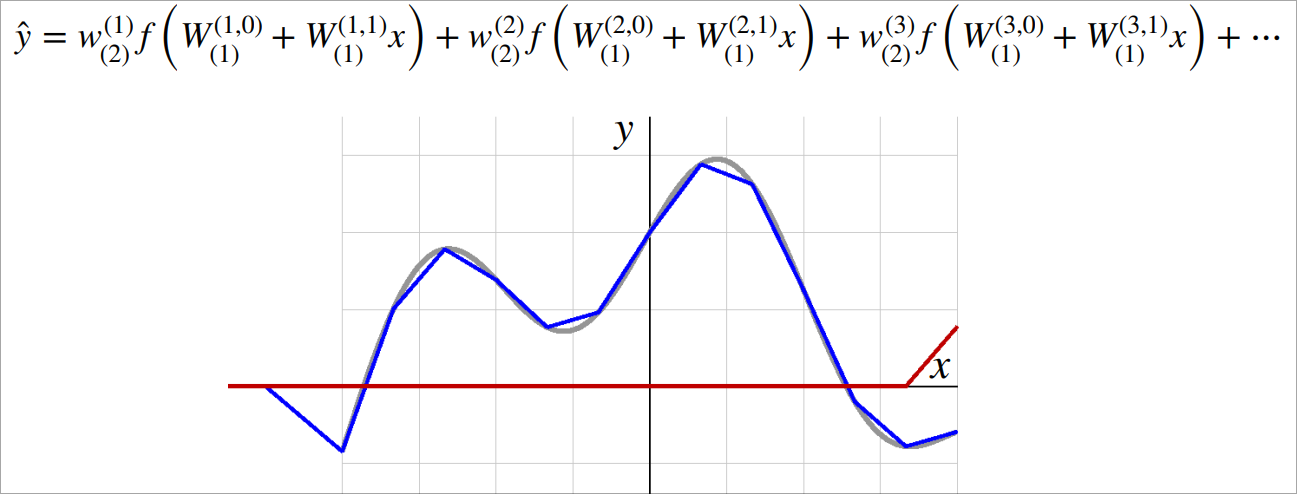
\includegraphics[scale=0.25]{screenshots/2026-04-21_1.png}
	\end{center}
\end{parag}



\begin{parag}{Dealing with multiple input dimensions}
	Handling $D > 1$ input dimensions makes very little different in the model formulation. From the 1D input formulation we had 
	\begin{align*} 
		\hat{y} = w_{\left(2\right)}^{T}f\left(W_{\left(1\right)}^{T}\begin{pmatrix} 1 \\ x \end{pmatrix} \right)
	\end{align*}
	In order to add dimensions -- to the $D$ case  we literally add the dimension in $W_{\left(1\right)}$ which now is of dimension $\left(D + 1\right) \times M$ instead of $2 \times M$. (where $x \in \mathbb{R}^{D + 1}$).
    
\end{parag}


\begin{parag}{Dealing with multiple output dimensions}
    To handle $C > 1$ output dimensions, we can proceed as in the case of linear models. We simply need to replace the vector of parameters $w_{\left(2\right)}$ with a matrix $W_{\left(2\right)} \in \mathbb{R}^{M \times C}$. Therefore this prediction can be written as 
	\begin{align*} 
		\hat{y} = W_{\left(2\right)}^{T}f\left(W_{\left(1\right)}^{T}x\right)
	\end{align*}
\end{parag}


\begin{parag}{Simple artificial neural network}
    The resulting simple artificial neural network with one hidden layer can be depicted as shown below.
\end{parag}

\begin{figure}[h!]
    
	\centering

\begin{tikzpicture}[
    node distance = 0pt,
    neuron/.style = {
        circle,
        draw=black,
        minimum size = 22pt,
        inner sep = 0pt,
        line width = 0.8pt
    },
    >=Stealth
]

%% ── Column x-positions ──────────────────────────────────────────────────────
\def\xIn{0}
\def\xHid{3.6}
\def\xOut{7.2}

%% ── INPUT LAYER ─────────────────────────────────────────────────────────────
%  7 nodes: bias(1), x^(1)…x^(3), vdots, x^(D-1), x^(D)
\node[neuron] (i0)  at (\xIn, 0)     {$1$};
\node[neuron] (i1)  at (\xIn,-1.1)   {$x^{(1)}$};
\node[neuron] (i2)  at (\xIn,-2.2)   {$x^{(2)}$};
\node[neuron] (i3)  at (\xIn,-3.3)   {};   % spare visible node
\node         (id)  at (\xIn,-4.15)  {$\vdots$};
\node[neuron] (i4)  at (\xIn,-5.2)   {};
\node[neuron] (i5)  at (\xIn,-6.3) {$x^{(D)}$};

% label x^(3) and x^(D-1) inside the plain nodes
\node at (i3) {$x^{(3)}$};

%% ── HIDDEN LAYER ─────────────────────────────────────────────────────────────
%  6 nodes: top z^(1)_(1) … bottom z^(M)_(1)
\node[neuron] (h1) at (\xHid,-0.6)  {$z_{(1)}^{(1)}$};
\node[neuron] (h2) at (\xHid,-1.7)  {};
\node[neuron] (h3) at (\xHid,-2.8)  {};
\node[neuron] (h4) at (\xHid,-3.9)  {};
\node[neuron] (h5) at (\xHid,-5.0)  {};
\node[neuron] (h6) at (\xHid,-6.1)  {$z_{(1)}^{(M)}$};

%% ── OUTPUT LAYER ─────────────────────────────────────────────────────────────
%  4 nodes: ŷ^(1), two blanks, ŷ^(C)
\node[neuron] (o1) at (\xOut,-1.5)  {$\hat{y}^{(1)}$};
\node[neuron] (o2) at (\xOut,-2.7)  {};
\node         (od) at (\xOut,-3.7)  {$\vdots$};
\node[neuron] (o3) at (\xOut,-4.7)  {};
\node[neuron] (o4) at (\xOut,-5.9)  {$\hat{y}^{(C)}$};

%% ── WEIGHTS: input → hidden ──────────────────────────────────────────────────
\foreach \i in {i0,i1,i2,i3,i4,i5}{
  \foreach \h in {h1,h2,h3,h4,h5,h6}{
    \draw[black, line width=0.4pt] (\i) -- (\h);
  }
}

%% ── WEIGHTS: hidden → output ─────────────────────────────────────────────────
\foreach \h in {h1,h2,h3,h4,h5,h6}{
  \foreach \o in {o1,o2,o3,o4}{
    \draw[black, line width=0.4pt] (\h) -- (\o);
  }
}

%% ── OUTPUT ARROWS ─────────────────────────────────────────────────────────────
\draw[->, line width=0.8pt] (o1.east) -- ++(0.8,0) node[right] {$\hat{y}^{(1)}$};
\draw[->, line width=0.8pt] (o4.east) -- ++(0.8,0) node[right] {$\hat{y}^{(C)}$};

%% ── COLUMN HEADERS ───────────────────────────────────────────────────────────
\node[above=18pt of i0, font=\large\bfseries] {$\mathbf{x}$};
\node[above=4pt  of i0, font=\small]          {input layer};

\node[above=18pt of h1, font=\large\bfseries] {$\mathbf{z}_{(1)}$};
\node[above=4pt  of h1, font=\small]          {hidden layer};

% output-layer header sits above o1 and to the right
\node[above=18pt of o1, font=\large\bfseries] {$\hat{\mathbf{y}}$};
\node[above=4pt  of o1, font=\small]          {output layer};

\end{tikzpicture}
\caption{Artificial neural networks which I passed a bit too much time on}
\end{figure}


\begin{parag}{$ $}
    

	Because we use a matrix vector product for each layer, the layers are called fully connected.
\end{parag}

As we can see here, even with a single hidden layer, one can already model complicated functions. The \important{Universal approximation theorem} states that a sufficiently large feed forward network with a non-linear activation can approximate any continuous function on a compact domain to arbitrary precision. But why stop at just one hidden layer?


\begin{parag}{Multilayer Perceptron}
	In essence, we could just '\textit{stack}' horizontally layer of layer of neural network to construct a bigger one. This is what the Multilayer Perceptron does. 
	\begin{itemize}
		\item For the first hidden layer, we still have 
			\begin{align*} 
				z_{\left(1\right)} =  f\left(W_{\left(1\right)}^{T}x\right)
			\end{align*}
			\item For any subsequent layer $l$, we have 
				\begin{align*} 
					z_{\left(l\right)} = f\left(W_{\left(l\right)}^{T}z_{l - 1}\right)
				\end{align*}
				\item Finally, for a network of $L$ layer, we compute the output as 
					\begin{align*} 
						\hat{y} = W_{\left(L\right)}^{T}z_{\left(L - 1\right)}
					\end{align*}
				The process of going from the input to the output is called the \important{forward pass} of the network
	\end{itemize}
	If we wanted to write the prediction as a single equation it would look like:
	\begin{align*} 
		\hat{y} =  W_{\left(L\right)}^{T}f\left(W_{\left(L - 1\right)}^{T}f\left(W_{L - 2}^{T}f\left(\cdots f\left(W_{\left(1\right)}^{T}x\right)\right)\cdots\right)\right)
	\end{align*}
    This is not very convenient, and it is easier to simply think of $\hat{y}$ as a function of all parameters
	\begin{align*} 
		\hat{y} = \hat{y}\left(W\right)
	\end{align*}
	Where $W =  \left\{W_{\left(l\right)}\right\}$ encompasses the parameters of all the layers.
\end{parag}

Our model has been define and it looks very good on paper however there is still a big issue, the \important{training}. Given a set of $N$ training sample $l\left(x_i, y_i\right)$, we would then like to find the best set of parameters $W^{\ast}$. As usual this is done by minimizing an empirical risk w.r.t. all the parameters $W$.\\
$ $ \\
For regression, the loss function is typically the square loss 
\begin{align*} 
	R\left(W\right) = \frac{1}{N} \sum_{i= 1}^{N}\left\|\hat{y}_i\left(W\right) - y_i\right\|^2
\end{align*}
Where the dependence of $\hat{y}_i $ on the parameters $W$ is denoted as in the previous slide.


\begin{parag}{Training an MLP}
    Because an MLP stacks multiple layers, each of which has a nonlinear activation function, the problem does not have a closed form solution and is not convex\\
	$ $\\
	Learning is therefore done by gradient descent. While the gradient might seem complicated, it can in fact be computed in a nice manner (this is called backpropagation).
\end{parag}

\begin{parag}{Gradient based learning}
    Because the empirical risk is an average over the training samples, its gradient will also be an average of gradients. Thus we can focus on a single loss term $l\left(\hat{y}_i , y_i\right)$, where 
	\begin{align*} 
		R\left(\left\{W_{\left(l\right)}\right\}\right) = \frac{1}{N}\sum_{i= 1}^{N}l\left(\hat{y}_i, y_i\right)= \frac{1}{N}\sum_{i= 1}^{N}l_i
	\end{align*}
	For simplicity, we will assume that all hidden layers use the same type of activation function, denoted by $f$.\\
	$ $\\
	For the $k^{\text{th}}$ dimension of the output of any layer $l$, let us define 
	\begin{align*} 
		a_{\left(l\right)}^{\left(k\right)} =  \sum_{j} W_{\left(l\right)}^{\left(k, j\right)} z_{\left(l - 1\right)}^{\left(j\right)}
	\end{align*}
	Which denotes the dot product between the $k^{\text{th}}$ column of $W_{\left(l\right)}$ and $z_{\left(l-1\right)}$. What we aim to compute is the derivative of the loss function $l_i$ w.r.t. any parameter $W_{\left(l\right)}^{\left(k, j\right)}$. An important thing here to understand is what is $W_{\left(l\right)}^{\left(k, j\right)}$ recall that this \important{an element} of the parameter of the model at the layer $l$, the parameter at the column k and row j. Following the chain rule, we can write such a derivative as 
	\begin{align*} 
		\frac{\partial l_i}{\partial W_{\left(l\right)}^{\left(k, j\right)}} = \frac{\partial l_i}{\partial a_{\left(l\right)}^{\left(k\right)}}  \frac{\partial a_{\left(l\right)}^{\left(k\right)}}{\partial W_{\left(l\right)}^{\left(k, j\right)}} 
	\end{align*}


	As the definition stated above, we can see that 
	\begin{align*} 
		\frac{\partial a_{\left(l\right)}^{\left(k\right)}}{\partial W_{\left(l\right)}^{k, j}} = z_{l - 1}^{\left(j\right)}
	\end{align*}
	Furthermore, let us define 
	\begin{align*} 
		\delta_{\left(l\right)}^{\left(k\right)} =  \frac{\partial l_i}{\partial a_{\left(l\right)}^{\left(k\right)}} 
	\end{align*}
	Which directly encodes the first term of the derivative. So now we can rewrite the derivative 
	\begin{align*} 
		\frac{\partial l_i}{\partial W_{\left(l\right)}^{\left(k, j\right)}}  = \delta_{\left(l\right)}^{\left(k\right)}z_{\left(l-1\right)}^{\left(j\right)}
	\end{align*}
	\begin{subparag}{Little break}
		Remainder here to pause and check if I understood everything here.
	\end{subparag}
	Because the hidden values $\left\{z_{l -1}^{\left(j\right)}\right\}$ are computed in the forward pass, we only need to compute the $\left\{\delta_{\left(l\right)}^{\left(k\right)}\right\}$ to obtain the derivative of the loss w.r.t. any parameter.\\
	$ $\\
	For the last layer (Layer $L$), we have (assuming no final activation)
	\begin{align*} 
		a_{\left(L\right)}^{\left(k\right)} = \hat{y}^{\left(k\right)}
	\end{align*}
	This means that, for the last layer, $\delta_{\left(L\right)}^{\left(k\right)}$ can be computed explicitly as the partial derivative of the loss function w.r.t. the network's output. E.g., for the square loss, we have 
	\begin{align*} 
		\delta_{\left(L\right)}^{\left(k\right)} =  2\left(\hat{y}_i^{\left(k\right)} - y_i^{\left(k\right)}\right)
	\end{align*}
	Therefore for all other layers where $l < L$, it can be shown that $\delta_{\left(l\right)}^{\left(k\right)}$ can be computed from:
	\begin{itemize}
	    \item the $\left\{\delta_{\left(l + 1\right)}^{\left(j\right)}\right\}$, from the subsequent layer $l + 1$ 
	    \item the derivative of the activation function w.r.t. its input
	    \item the parameters $W_{\left(l + 1\right)}$ (of the subsequent layer $l + 1$)
	\end{itemize}
	In other words, given $\delta_{\left(l + 1\right)}$, one can compute $\delta_{\left(l\right)}$. And as we can explicitly compute $\delta_{\left(L\right)}$ for the last layer, using recursion, we can then compute $\delta$ for any layer. Using this fact we get that in order to compute the gradient, we can compute 
	\begin{align*} 
		\frac{\partial l_i}{\partial W_{\left(l\right)}^{\left(k, j\right)}}  = \delta_{\left(l\right)}^{\left(k\right)}z_{\left(l-1\right)}^{\left(j\right)}
	\end{align*}
	The algorithm works for computing the gradient at any layer. To do so we start from the last one:
	\begin{enumerate}
	    \item Propagate $x_i$ forward through the network
	    \item Compute $\delta_{\left(L\right)}$ depending on the loss
	    \item Propagate $\delta_{\left(L\right)}$ backward to obtain each $\delta_{\left(l\right)}$
	    \item At each layer, compute the partial derivatives
			\begin{align*} 
				\frac{\partial l_i}{\partial W_{\left(l\right)}^{\left(k, j\right)}} = \delta_{\left(l\right)}^{\left(k\right)}z_{\left(l - 1\right)}^{\left(j\right)}
			\end{align*}
			Where $z_{\left(l - 1\right)}$ has been computed during the forward pass. Recall that $z_{\left(l - 1\right)}$ represent the value at the given layer.
	\end{enumerate}
	
\end{parag}




\subsection*{Little example on auto differentiation (not in the course)}

Something that I want to emphasize here (that I found not clear) is what are we even doing here. So to explain a bit more I will use the lecture about autodiff from cs-328. What we were doing above was auto differentiation, there is two main modes \important{forward}, \important{backward}. The one we saw above is backward. How it works is first execute the program and store each result into a tape (this is our $z_{\left(i\right)}$ above). Then we go back and compute the differentiation using that tape:
\begin{center}
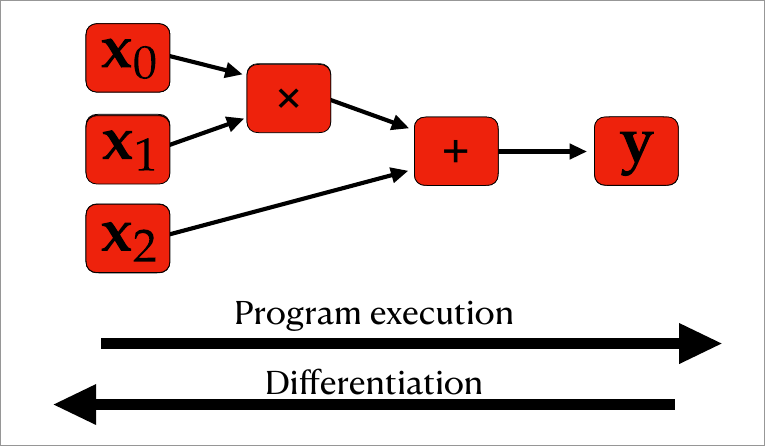
\includegraphics[scale=0.3]{screenshots/2026-04-21_3.png}
\end{center}
Do later
\\


\begin{parag}{Gradient descent}
    Once the gradient is computed, the update at iteration $k$ is performed as 
	\begin{align*} 
		W_k \leftarrow W_{k-1} - \mu \nabla_W R\left(W_{k-1}\right)
	\end{align*}
	Where $W$ encompasses the parameters of all layers\\
	$ $\\
	You can also think of this as updating the parameters in each layer $l$ as 
	\begin{align*} 
		W_{\left(l\right), k} \leftarrow W_{\left(l\right), k - 1} - \mu \nabla_{W_{\left(l\right)}}R\left(W_{k - 1}\right)
	\end{align*}
	Where $W_{\left(l\right), k}$ represents the parameters of layer $l$ at iteration $k$ of gradient descent.\\
	$ $\\
	The empirical risk is the average of the loss function value over all training samples. Because the gradient of an average is the average of the gradients. We can write also a standard gradient update as 
	\begin{align*} 
		W_{k} \leftarrow W_{k-1} - \mu \frac{1}{N}\sum_{i= 1}^{N}\nabla_W l_i\left(W_{k-1}\right)
	\end{align*}
	this means that, for each gradient descent iteration, one needs to perform a forward pass and a backward pass through the network for all the training samples. This becomes expensive for large training sets. 
\end{parag}

\begin{parag}{Stochastic gradient descent}
    A way in order to solve this issue is to not use all the training set when doing a gradient descent. But a big issue comes to us: Which subset should we take? Let us take a random subset of our data set right? But how small, at this point let us just take one random point and do the iterations of the gradient descent on only one point. This is called \important{Stochastic gradient descent}.
	\begin{subparag}{Definition}
	    \important{Stochastic gradient descent} updates the parameters $W$ based on the gradient of a single sample in each iteration 
		\begin{align*} 
			W_{k} \leftarrow W_{k-1} - \mu \nabla l_{i\left(k\right)} \left(W_{k-1}\right)
		\end{align*}
		At each iteration, we use the gradient of a single loss term. The index of the sample depends on the iteration number $k$.
	\end{subparag}
	In practice, one then iterates over the training samples, either in fixed order or in a random one.
\end{parag}

\begin{parag}{SGD with mini-batches}
    The gradient obtained by a single sample might be a poor approximation of the true, complete gradient. To obtain more reliable gradient estimate, one typically uses mini-batches of $B$ samples (this is what we said above). The parameters are then updated as 
	\begin{align*} 
		W_{k} \leftarrow W_{k-1} - \mu \sum_{b= 1}^{B} \nabla l_{i\left(b, k\right)} \left(W_{k-1}\right)
	\end{align*}
	The index of the samples used for the update now depends on the iteration number $k$ and on the index $b$ of the samples in the mini-batch
\end{parag}




\begin{parag}{Simple network training: Regression example}
	The example that we will take now is a model which takes as input a 2D coordinate and output a 1D coordinate. The function that we are trying to model is given by 
	\begin{align*} 
		y = 100\left(x^{\left(2\right)} - \left(x^{\left(1\right)}\right)^2\right)^2 + \left(1 - x^{\left(1\right)}\right)^2
	\end{align*}
	\begin{center}
	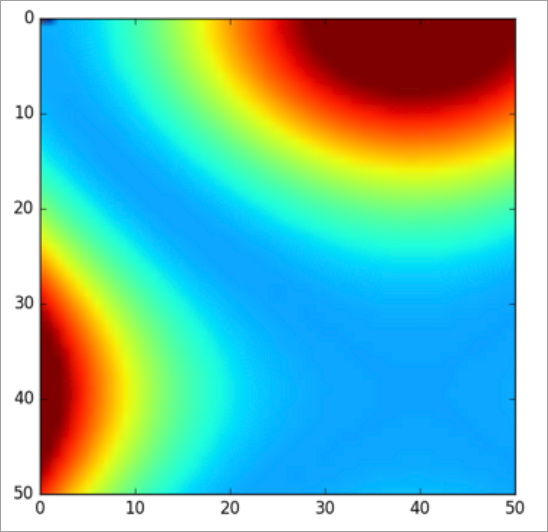
\includegraphics[scale=0.2]{screenshots/2026-04-22.png}
	\end{center}
	We will try different models, respectively with 2, 3, 4 nodes which gives us:
	\begin{center}
	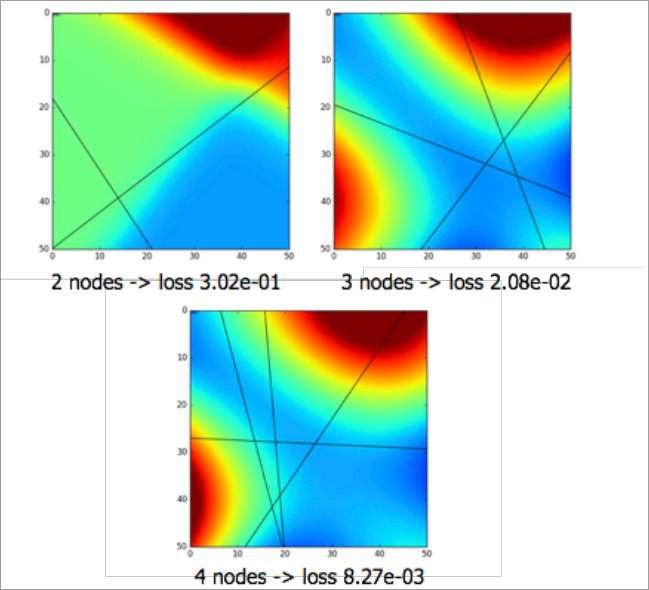
\includegraphics[scale=0.2]{screenshots/2026-04-22_1.png}
	\end{center}
	\begin{subparag}{Nodes}
	    Just to have more context a node (also called a neuron or unit) is a single computational element. Formally, it take an input vector $x$, computes an affine transformation $w^{T}x + b$, and then applies a nonlinearity (e.g., ReLU, sigmoid). So one node corresponds to one scalar output.\\
	\end{subparag}
	An example that allows us to have a better intepretation on how does neuron will do is to use the surface/output 
	\begin{align*} 
		y = \sin\left(x^{\left(1\right)}\right)\sin\left(x^{\left(2\right)}\right)
	\end{align*}
	\begin{center}
	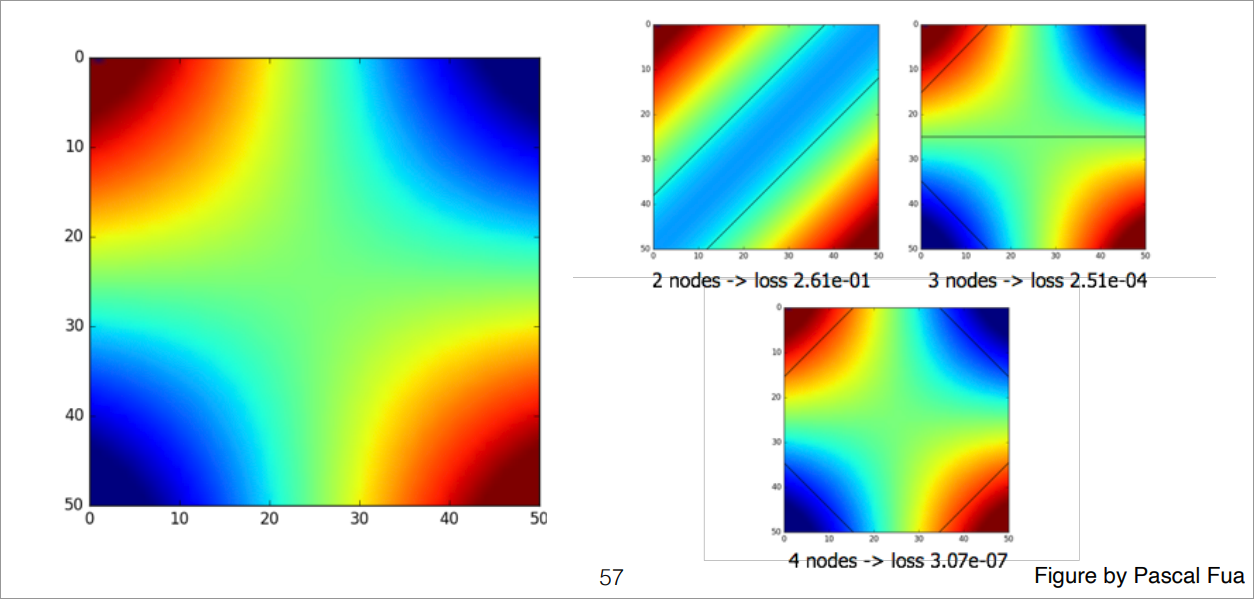
\includegraphics[scale=0.25]{screenshots/2026-04-22_2.png}
	\end{center}
	However even if here in this case we see why it works, usually we don't actually know why they work, meaning that we don't know:
	\begin{itemize}
	    \item What do the coefficients actually mean?
	    \item Will the network generalize to other simulations
	    \item Why does the training process actually work?
	\end{itemize}
	What we know:
	\begin{itemize}
	\item How all the coefficients were obtained (as it is a deterministic calculation after all)
	\item Which neural network components work well, and which of them work well together
	\end{itemize}
\end{parag}




\begin{parag}{SGD behaviour}
    Because it approximates the full gradient, SGD will move the parameters less directly towards a local minimum.
	\begin{itemize}
		\item The parameters dance around the minimum, which may require decreasing the learning rate
		\item Nevertheless, SGD can help to avoid bad local minima
	\end{itemize}
	\begin{center}
	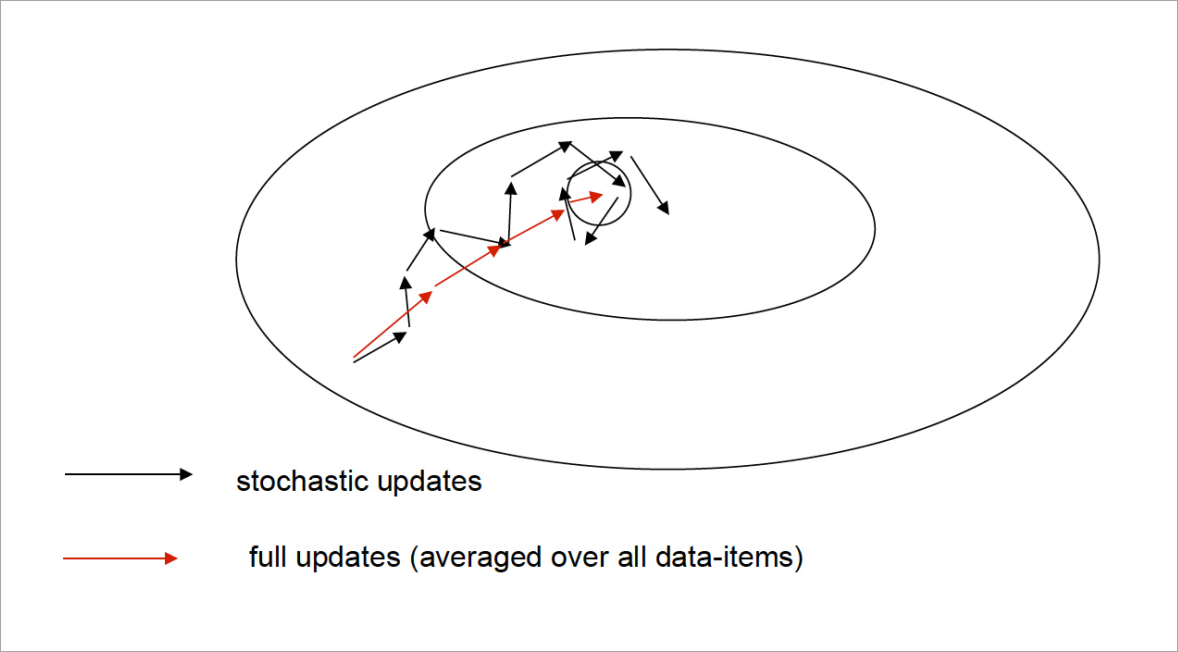
\includegraphics[scale=0.28]{screenshots/2026-04-22_3.png}
	\end{center}
	To illustrate how '\textit{important}' using mini batch is when doing gradient descent based optimization, let us see this graph
	\begin{center}
	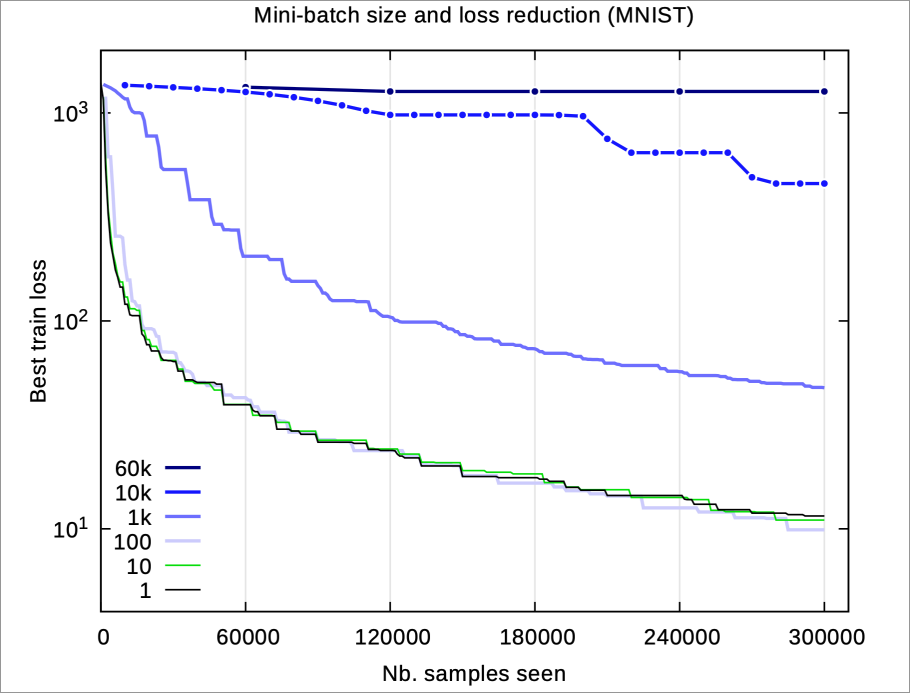
\includegraphics[scale=0.24]{screenshots/2026-04-22_4.png}
	\end{center}
	
\end{parag}


\begin{parag}{Gradient descent: Limitations}
    Gradient descent makes strong assumption about the magnitude and isotropy of the local curvature so that the same step size can be used in all directions. What we mean by that is that in order for our algorithm to work well we need our function to behave nicely. (there is a couple of example of gradient descent in the slide p.64 lecture 9). For instance imagine if we have a very local minima then our function might get stuck there instead of rolling out away. What we are lacking here is \important{momentum}
\end{parag}

\begin{parag}{SGD Extension}
    The idea we have is to add inertia to the parameter updates 
	\begin{align*} 
		\nu \leftarrow \gamma \nu + \mu \nabla R\left(W\right)\\
		W \leftarrow W - \nu
	\end{align*}
	With $\gamma > 0$, the moment accelerates if the gradient does not change too much.\\
	$ $\\
	As you could have guessed there is a lot of SGD extensions our there some uses adaptive learning rate:
	\begin{itemize}
		\item Adagrad (Duchi et al, JMLR 2011)
		\item Adadelta (Zeiler, 2012)
		\item RMSprop (Hinto, 2012)
		\item ADAM (Kingma et al., ICLR 2015)
	\end{itemize}
	For example, ADAM uses a moving average of each coordinate to rescale each coordinate separately.
	\begin{center}
	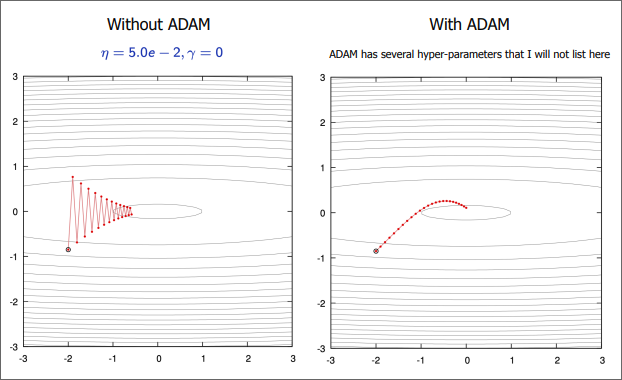
\includegraphics[scale=0.3]{screenshots/2026-04-22_5.png}
	\end{center}
\end{parag}


\begin{parag}{Gradient vanishing \& Initialization}
    The activation functions often have saturating regions where the gradient becomes (close to ) $0$
	\begin{center}
	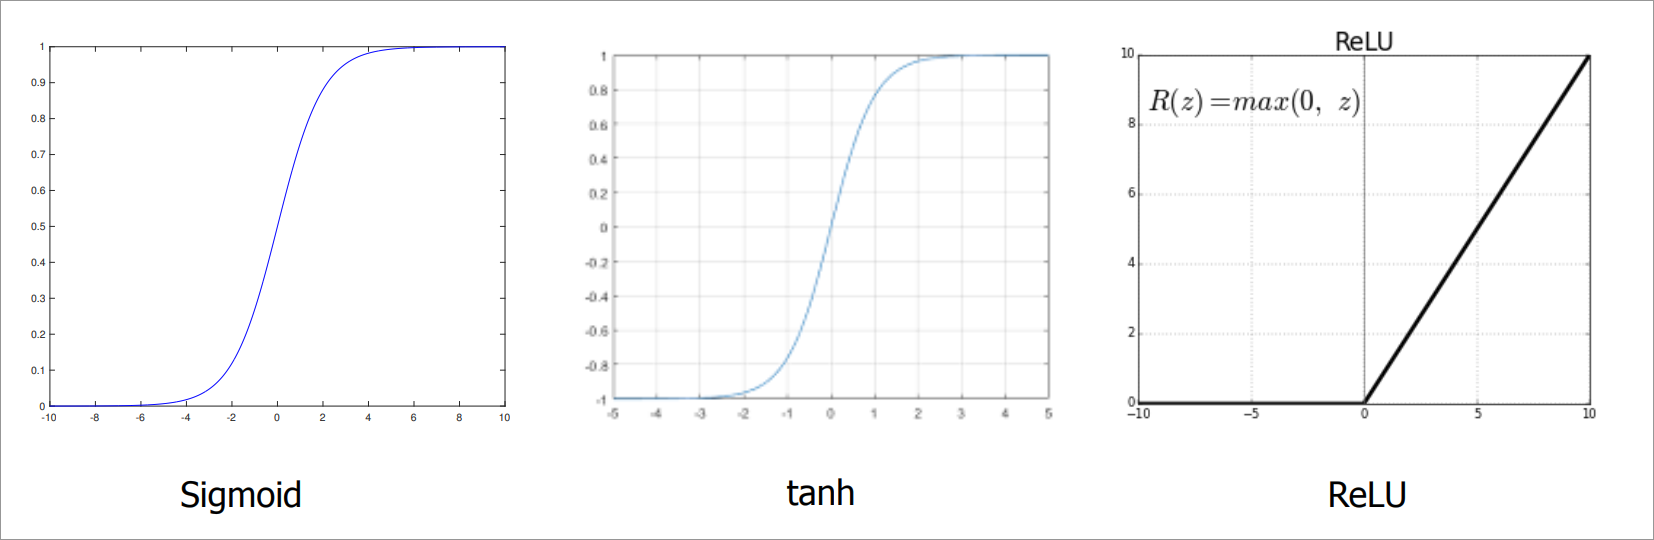
\includegraphics[scale=0.25]{screenshots/2026-04-22_6.png}
	\end{center}
	Glorot and Bengio observed that the gradient vanishes exponentially with the (inverse) depth if the weights are such that they tend to often saturate the activation function. '\textit{saturate the activation function}' refers to regions where the derivative is very small (e.g., sigmoid saturates near 0 or 1, $\tanh$ near -1 or 1). Now let us go back to backpropagation. Gradients are computed using the chain rule. For a deep network with $L$ layers, a gradient term typically looks like a product:
	\begin{align*} 
		\frac{\partial \mathcal{L}}{\partial x} = \prod_{l= 1}^{L}\frac{\partial x^{\left(l\right)}}{\partial z^{\left(l-1\right)}} 
	\end{align*}
	Each factor contains a weight matrix and the derivative of the activation function. If this activation is saturated, those derivative are small number. So we end up multiplying $0.1 \cdot  0.1 \cdot 0.1 \cdot \cdots$. This shrinks exponentially with depth. The gradient becomes extremely close to $0$ as the number of layers increases.\\
	$ $\\
	To overcome this, Glorot and Bengio introduced a weight initialization strategy where the range of the initial random values of the weights is layer dependent.
\end{parag}







\begin{parag}{From regression to classification}
    So far, we have focused on the case where the prediction is taken directly as the output of a linear model applied to the last hidden representation, i.e.,
	\begin{align*} 
		\hat{y} = W_{\left(L\right)}^{T}z_{\left(L-1\right)}
	\end{align*}
	While this is fine for regression task, it is not ideal for a classification one, where we would like each $\hat{y}^{\left(k\right)}$ to represent the probability (score) for class $k$. This can be achieved via the softmax function (as in multi-class logistic regression)
	\begin{align*} 
		\hat{y}^{\left(k\right)} = \frac{\exp\left(w_{\left(L\right)\left(k\right)}^{T}z_{L-1}\right)}{\sum_{j= 1}^{C}\exp\left(w_{\left(L\right)\left(j\right)}^{T}z_{\left(L-1\right)}\right)}
	\end{align*}
	Where $w_{\left(L\right)\left(j\right)}$ indicates the j$\Th$ column of $W_{\left(L\right)}$.\\
	$ $\\
	In this case, the empirical risk is typically defined as the cross entropy
	\begin{align*} 
		R\left(W\right) = -\frac{1}{N}\sum_{i= 1}^{N}\sum_{k= 1}^{C}\hat{y}_i^{\left(k\right)}\ln \hat{y}_i^{\left(k\right)}
	\end{align*}
	Backpropagation then requires computing the derivative of the cross-entropy w.r.t. each $\hat{y}^{\left(k\right)}$ and the derivative of the softmax function w.r.t. each $W_{\left(L\right)}^{\left(j, k\right)}$.
	\begin{subparag}{Remark}
	    Note that this is similar to the derivatives computed for multi-class logistic regression.
	\end{subparag}
\end{parag}



\begin{parag}{Working with images}
    Treating an images as a big vector seems counter-intuitive. 
	\begin{itemize}
		\item An image of reasonable size yield a huge vector, thus a huge amount of parameters in an MLP
		\item Small image regions have similar property and should not be processed independently
		\item A translation should not affect results
	\end{itemize}
	
\end{parag}













